\documentclass[a4paper, 12pt]{article}
\usepackage{geometry}
\usepackage{graphicx}

\usepackage{fancyhdr}
\pagestyle{fancy}
\fancyhf{}
\rhead{Kevin Wallis}
\lhead{Dokumentation Travelling Salesman}
\rfoot{Page \thepage}

\begin{document}

\section*{Allgemein}
Die Programmieraufgabe wurde in C\# mit Verwendung von WPF gelöst. Es wurde auf Frameworks wie \textit{MEF}, \textit{Prism} oder \textit{PostSharp} verzichtet. Dadurch ist die Anwendung sehr gut verst\"andlich. Zur L\"osung des Travelling Salesman Problems (TSP) wurde ein Simulated Annealing Algorithmus mit Standardwerten verwendet und zur Kontrolle Brute Force. Zudem bietet die Anwendung die M\"oglichkeit eigene Algorithmen zu implementieren, dazu muss von einer bestehenden Klasse (\textit{Algorithm}) abgeleitet sowie eine Methode implementiert werden.\\
Bei Fragen stehen ich Ihnen gerne zur Verfügung: \textit{kevin.wallis@hotmail.com}

\section*{Setup}
Um das Programm ausf\"uhren zu k\"onnen, muss das \textit{.Net Framework} auf dem Computer installiert sein. Es gibt einen Ordner \textit{Setup}, dort ist die Anwendung (\textbf{TravellingSalesman.exe}) und drei Testdateien (\textbf{TestA}, \textbf{TestB} und \textbf{TestC}) enthalten. Die Anwendung kann mittels Doppelklick ge\"offnet werden und sollte ohne Weiteres starten. Der Source-Code ist einem Extra-Ordner (\textit{Source}) enthalten.

\section*{Funktionalit\"at}
Wie bereits erw\"ahnt wurde ein Simulated Annealing Algorithmus sowie Brute Force implementiert. Die Anwendung ist in Abbildung~\ref{fig:main_page} ersichtlich. Insgesamt gibt es zwei Tab Pages, die Main Page, hier werden einerseits die Punkte verwaltet und andererseits die Optimierungen gestartet. In der zweiten Page sind die Statistiken ersichtlich und mittels Klick auf eine Statistik, wird der Pfad aufgezeigt (siehe Abbildung~\ref{fig:statistics_page}). Im Folgenden werden ein paar Punkte zur Hauptansicht gelistet: 

\begin{itemize}
\item Es kann zwischen zwei Algorithmen gewechselt werden (Simulated Annealing und Brute Force).
\item Neben dem Algorithmus werden Tourendistanz und Laufzeit angezeigt.
\item In der Liste k\"onnen die Punkte bearbeitet werden, solange die Anwendung nicht l\"auft. Jede Bearbeitung wird sofort in der Grafik aktualisiert.
\item Der ausgew\"ahlte Punkt aus der Liste wird rot in der Grafik dargestellt.
\item Mittels Klick auf den M\"ulleimer (rechts oben), wird der ausgew\"ahlte Punkt gel\"oscht und die Grafik neu verbunden.
\item Durch die Eingabe einer X und einer Y Koordinate k\"onnen neue Punkte definiert werden (der Button mit dem Plus best\"atigt das Hinzuf\"ugen). Hierbei ist zu beachten, dass nur Zahlen zwischen 0 und 500 (inklusive) eingegeben werden k\"onnen, Buchstaben werden nicht angenommen.
\item Ein Ausf\"uhrung kann mit Klicken auf den gr\"unen Knopf gestartet werden.
\item W\"ahrend der Ausf\"uhrung wechselt der gr\"une Knopf zu rot und bei erneutem Klicken bricht die Optimierung ab.
\item Jeder Abbruch einer Ausf\"uhrung erzeugt eine Statistik, gleiches gilt auch, wenn der Algorithmus selbstst\"andig beendet wird.
\item Die Anwendung bietet die Option eine bestehende Landschaft (Punkte) zu speichern und sp\"ater wieder zu laden.
\end{itemize}

\begin{figure}[tbh]
    \centering
    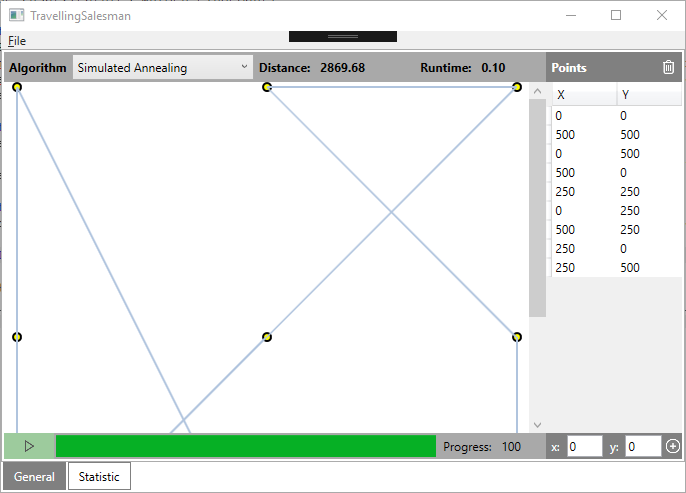
\includegraphics[width=0.8\textwidth]{mainPage}
    \caption{Main Page}
    \label{fig:main_page}
\end{figure}

\begin{figure}[tbh]
    \centering
    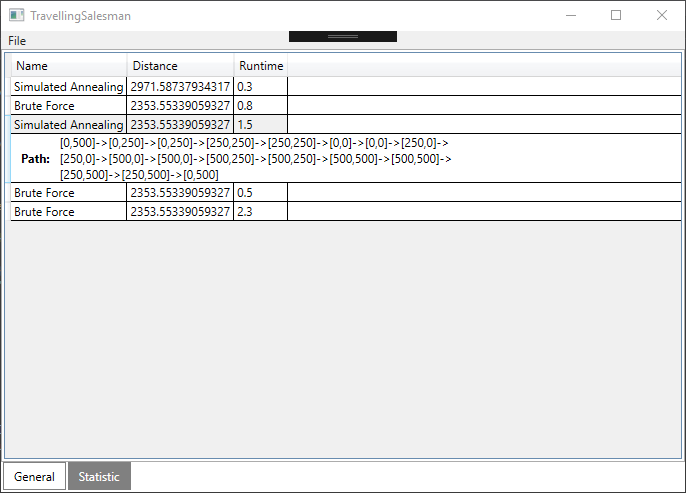
\includegraphics[width=0.8\textwidth]{statisticsPage}
    \caption{Statistics Page}
    \label{fig:statistics_page}
\end{figure}

\end{document}